\documentclass[11pt,a4paper]{book}

% --- CARGA DEL PAQUETE DE ESTILO PERSONALIZADO ---
\usepackage{core/jlrisco-tfx}

% --- DEFINICIÓN DE CONSTANTES DEL DOCUMENTO ---
\newcommand{\miAutor}{Ana Isabel García Fernández}
\newcommand{\miDirector}{José Luis Risco Martín}
% Si hubiese más directores los añadimos separados por " \\ ", ejemplo:
%\newcommand{\miDirector}{José Luis Risco Martín \\ Segundo Esteban San Román}
\StrSubstitute{\miDirector}{\\}{y}[\miDirectorInline]
\newcommand{\miTituloES}{Diseño y Optimización de un Sistema Empotrado de Bajo Consumo para la Detección de Anomalías en Tiempo Real mediante TinyML}
\newcommand{\miTituloEN}{Design and Optimization of a Low-Power Embedded System for Real-Time Anomaly Detection using TinyML}
\newcommand{\miTFX}{Trabajo de Fin de Máster}
%\newcommand{\miTFX}{Trabajo de Fin de Grado}
\newcommand{\miCurso}{2025--2026}
\newcommand{\misEstudios}{Máster en Ingeniería Informática}
%\newcommand{\misEstudios}{Grado en Ingeniería Informática}
\newcommand{\miTFXyEstudios}{Trabajo de Fin de Máster en Ingeniería Informática}
%\newcommand{\miTFXyEstudios}{Trabajo de Fin de Grado en Ingeniería Informática}
\newcommand{\miDepartamento}{Departamento de Arquitectura de Computadores y Automática}
\newcommand{\miConvocatoria}{Junio 2026}
\newcommand{\miNota}{10}
\newcommand{\miCalificacion}{Matrícula de Honor}
\newcommand{\miFecha}{21 de julio de 2026}
\newcommand{\miDedicatoria}{A mis padres por haber creído en mí desde el comienzo de mi etapa universitaria.}
% --- FIN DE CONSTANTES ---

% --- INICIALIZACIÓN DE GLOSARIOS ---
% Es necesario ejecutar estos comandos en el preámbulo del documento principal.
\makeglossaries
\loadglsentries{glosario}

% --- INICIO DEL DOCUMENTO ---
\begin{document}

\frontmatter

% ---------------------------- PÁGINA DE TÍTULO -----------------------------
\begin{titlepage}
\centering

\vspace*{1.75cm}

\rule{12cm}{1pt}

{\Large \textbf{\miTituloES} \par}
{\Large \textbf{\miTituloEN} \par} 

\rule{12cm}{1pt}

\vspace{0.75cm}

\includegraphics[width=4.25cm]{core/logo_ucm.png}
\vspace{0.75cm}

{\Large \textbf{\miTFX}} \\
{\Large \textbf{Curso~\miCurso} \par}

\vspace{1cm}
\vfill

{\Large \textbf{Autor}} \\
{\large \textbf{\miAutor} \par}

\vspace{0.25cm}

{\Large \textbf{Director}} \\
{\large \textbf{\miDirector} \par}

\vspace{0.25cm}

{\large \textbf{\misEstudios}}\\
{\large \textbf{Facultad de Informática}}\\
{\large \textbf{Universidad Complutense de Madrid}}

\end{titlepage}

% ---------------------------- SEGUNDA PÁGINA DE TÍTULO -----------------------------
\cleardoublepage
\thispagestyle{empty}
\begin{center}
\vspace*{1cm}

{\Huge {\miTituloES}} \\
{\Huge {\miTituloEN} \par}

\vspace*{2.5cm}

{\large \textbf{\miTFXyEstudios}} \\
{\large \textbf{\miDepartamento} \par}

\vspace{1cm}

{\Large \textbf{Autor}} \\
{\large \textbf{\miAutor} \par}

\vspace{0.50cm}

{\Large \textbf{Director}} \\
{\large \textbf{\miDirector} \par}

\vspace{0.75cm}\vfill

{\large \textbf{Convocatoria:}~\miConvocatoria}\\
{\large \textbf{Calificación:}~\miNota~(\miCalificacion)}

\vspace{1.00cm}\vfill

{\large \textbf{\misEstudios}}\\
{\large \textbf{Facultad de Informática}}\\
{\large \textbf{Universidad Complutense de Madrid} \par}
{\large \textbf{\miFecha}}
\end{center}

\chapter*{Autorización de difusión}
El abajo firmante, matriculado en el~\misEstudios~de la Facultad de Informática, autoriza a la Universidad Complutense de Madrid (UCM) a difundir y utilizar con fines académicos, no comerciales y mencionando expresamente a su autor el presente~\miTFX: ``\miTituloES'', realizado durante el curso académico~\miCurso~bajo la dirección de~\miDirectorInline~en el \miDepartamento, y a la Biblioteca de la UCM a depositarlo en el Archivo Institucional E-Prints Complutense con el objeto de incrementar la difusión, uso e impacto del trabajo en Internet y garantizar su preservación y acceso a largo plazo.

\vspace{5cm}

\begin{center}
\large \miAutor\\

\vspace{0.5cm}

\today
\end{center}

\chapter*{Dedicatoria}

\begin{flushright}
\begin{minipage}[c]{8.5cm}
\flushright{\textit{\miDedicatoria}}
\end{minipage}
\end{flushright}

\chapter*{Agradecimientos}
\lipsum[1-4]

\chapter*{Resumen}
\section*{\miTituloES}
\lipsum[1-4]

\section*{Palabras clave}   
\noindent Palabra Clave 1, Palabra Clave 2, Palabra Clave 3, Palabra Clave 4, Palabra Clave 5, Palabra Clave 6, Palabra Clave 7.

\chapter*{Abstract}
\section*{\miTituloEN}
\lipsum[1-4]

\section*{Keywords}
\noindent Keyword 1, Keyword 2, Keyword 3, Keyword 4, Keyword 5, Keyword 6, Keyword 7.

\tableofcontents 
\listoftables
\listoffigures
\lstlistoflistings

%Empiezan los capítulos de contenido
\mainmatter

%Intro
\chapter{Introducción}
Este capítulo sirve como un manual de referencia para utilizar las funcionalidades de \LaTeX{} incorporadas en esta plantilla. El objetivo es facilitar la redacción del documento, asegurando un formato consistente y profesional para las citas bibliográficas, figuras, tablas, ecuaciones, etc. A continuación, se detalla el procedimiento para cada uno de estos elementos.

\section{Citas y Referencias Bibliográficas}

La gestión de la bibliografía en este documento está automatizada mediante BibTeX. Todas las fuentes (artículos, libros, páginas web, etc.) deben ser añadidas al archivo \texttt{biblio.bib} que se encuentra en el directorio principal del proyecto.

\subsection{Añadir una nueva fuente}

Para añadir una nueva referencia, abre el archivo \texttt{biblio.bib} y añade una entrada con el formato BibTeX correspondiente. Cada entrada tiene un tipo (p.ej., \texttt{@article}, \texttt{@book}, \texttt{@misc}), una clave de cita única y varios campos con la información de la fuente.

Por ejemplo, para añadir una referencia a la API de simulación xDEVS, podrías añadir la siguiente entrada:
\begin{verbatim}
@article{RiscoMartin2023,
  title={x{DEVS}: {A} toolkit for interoperable modeling and simulation of 
         formal discrete event systems},
  author={Risco-Mart{\'\i}n, Jos{\'e} L and Mittal, Saurabh and Henares, Kevin 
          and Cardenas, Rom{\'a}n and Arroba, Patricia},
  journal={Software: Practice and Experience},
  volume={53},
  number={3},
  pages={748--789},
  year={2023},
  publisher={Wiley Online Library}
}
\end{verbatim}
La clave de cita en este caso es \texttt{RiscoMartin2023}, y es la que usaremos para referenciar esta fuente en el texto.

\subsection{Citar en el texto}

Una vez que la fuente está en el archivo \texttt{.bib}, puedes citarla en cualquier parte del documento usando el comando \verb|\cite{}|, introduciendo la clave de la cita dentro de las llaves. Por ejemplo:

El formalismo \gls{devs} permite modelar sistemas complejos mediante la descomposición en modelos atómicos y acoplados. Para implementar el modelo \gls{devs}, se utilizó la \gls{api} de simulación xDEVS~\cite{RiscoMartin2023}.

Si necesitas citar varias fuentes en el mismo punto, simplemente sepáralas por comas dentro del mismo comando \verb|\cite{}|. Por ejemplo:
\begin{verbatim}
...varios autores han tratado este tema \cite{Zeigler2018, RiscoMartin2023}.
\end{verbatim}

Que quedaría: varios autores han tratado este tema \cite{Zeigler2018, RiscoMartin2023}.

La bibliografía se generará automáticamente al final del documento, en la sección ``Bibliografía'', incluyendo todas las fuentes que hayas citado en el texto.

\section{Uso del Glosario y Acrónimos}

Para asegurar la claridad y consistencia del documento, la plantilla facilita el uso de un glosario y una lista de acrónimos gestionados por el paquete \texttt{glossaries}. Esto permite definir un término una sola vez y referenciarlo a lo largo del texto de forma automática.

\subsection{Definir un nuevo término}

Todos los términos, ya sean acrónimos o entradas de glosario, deben definirse en el fichero \texttt{glosario.tex}, que se carga automáticamente en el documento principal.

\subsubsection{Acrónimos}
Para añadir un nuevo acrónimo, utiliza el comando \verb|\newacronym|. Su estructura es: 
\begin{verbatim}
\newacronym{etiqueta}{acrónimo}{nombre completo} 
\end{verbatim}

La \texttt{etiqueta} es una clave única que usarás para referenciarlo en el texto.

Por ejemplo, para definir el acrónimo TFM:
\begin{verbatim}
\newacronym{tfm}{TFM}{Trabajo de Fin de Máster}
\end{verbatim}

También se puede definir un glosario, pero no es lo habitual en este tipo de trabajos. Por ello, solo usaremos la opción de crear y usar acrónimos.

\subsection{Citar términos en el texto}

Una vez definidos los términos en \texttt{glosario.tex}, puedes usarlos en el texto con los siguientes comandos. El paquete se encargará automáticamente de expandir el acrónimo la primera vez que se use y de utilizar solo la forma corta en las siguientes apariciones.

\begin{itemize}
    \item \verb|\gls{etiqueta}|: Es el comando principal. La primera vez que se usa, muestra el nombre completo seguido del acrónimo entre paréntesis. Por ejemplo, la primera vez que escribas \verb|\gls{tfm}|, aparecerá ``Trabajo de Fin de Máster (TFM)''. Las siguientes veces, solo aparecerá ``TFM''.

    \item \verb|\glspl{etiqueta}|: Se usa para la forma plural del término. Por ejemplo, \verb|\glspl{hems}| mostrará ``Home Energy Management Systems (HEMSs)'' la primera vez, y ``HEMSs'' después. En español hay que tener mucho cuidado con esto porque los acrónimos no tienen el mismo tratamiento que en inglés (el plural no se forma igual y además no suelen ir anticipadas por artículo) \cite{RAE-siglas}.

    \item \verb|\Gls{etiqueta}| y \verb|\Glspl{etiqueta}|: Son las versiones con mayúscula inicial, ideales para usar al principio de una frase.
\end{itemize}

Al final del documento, la lista de acrónimos y el glosario se generarán automáticamente, incluyendo solo los términos que hayas utilizado en el texto.


\section{Inclusión de Figuras}

Las figuras son un componente esencial para ilustrar conceptos, arquitecturas o resultados. Para una correcta organización del proyecto, se recomienda guardar todos los archivos de imagen en una subcarpeta dedicada, como por ejemplo la carpeta \texttt{fig/}, que ya se encuentra creada en esta plantilla.

Para insertar una figura en el documento, se utiliza el entorno \texttt{figure}. Este entorno gestiona la colocación de la imagen como un elemento flotante, aunque se puede forzar su posición con el especificador \texttt{[H]} (del paquete \texttt{float}) si se desea que aparezca exactamente en ese punto del texto\footnote{El uso de la opción \texttt{H} se desaconseja totalmente.}.

El siguiente código muestra cómo añadir una figura con su leyenda y prepararla para ser referenciada:

\begin{verbatim}
\begin{figure}
    \centering
    \includegraphics[width=0.8\textwidth]{fig/mi_figura.png}
    \caption{Este es el pie de foto que describe la figura.}
    \label{fig:mi_figura}
\end{figure}
\end{verbatim}

Los componentes clave de este bloque son:
\begin{itemize}
    \item \verb|\centering|: Centra la figura horizontalmente en la página.
    \item \verb|\includegraphics[width=...]{...}|: Es el comando que inserta la imagen. La opción \texttt{width} permite escalar la imagen a un ancho determinado (en el ejemplo, al 80\% del ancho de texto). La ruta del archivo apunta a la imagen que se desea incluir.
    \item \verb|\caption{...}|: Añade una leyenda descriptiva y numerada automáticamente debajo de la figura.
    \item \verb|\label{...}|: Asigna un identificador único a la figura. Es fundamental para poder referenciarla desde otras partes del documento. Se recomienda usar un prefijo como \texttt{fig:} para evitar confusiones con etiquetas de tablas, ecuaciones, etc.
\end{itemize}

Una vez que la figura ha sido etiquetada con \verb|\label|, puedes hacer referencia a ella en el texto de forma automática utilizando el comando \verb|\autoref{}|. Esta es la forma recomendada, ya que genera automáticamente el tipo de elemento y su número (p.ej., ``Figura 1.1'').

Por ejemplo, para citar la figura anterior, escribirías:
\begin{verbatim}
... la arquitectura del sistema se muestra en la \autoref{fig:mi_figura}.
\end{verbatim}

Al compilar el documento, LaTeX reemplazará \verb|\autoref{fig:mi_figura}| por ``Figura 1.1'' (o el número que corresponda), creando además un hipervínculo a la misma gracias al paquete \texttt{hyperref}. Por ejemplo:

En la \autoref{fig:diagrama_ejemplo} se ilustra el diagrama de bloques del sistema empotrado que se ha diseñado en este \gls{tfm}.

\begin{figure}
    \centering
    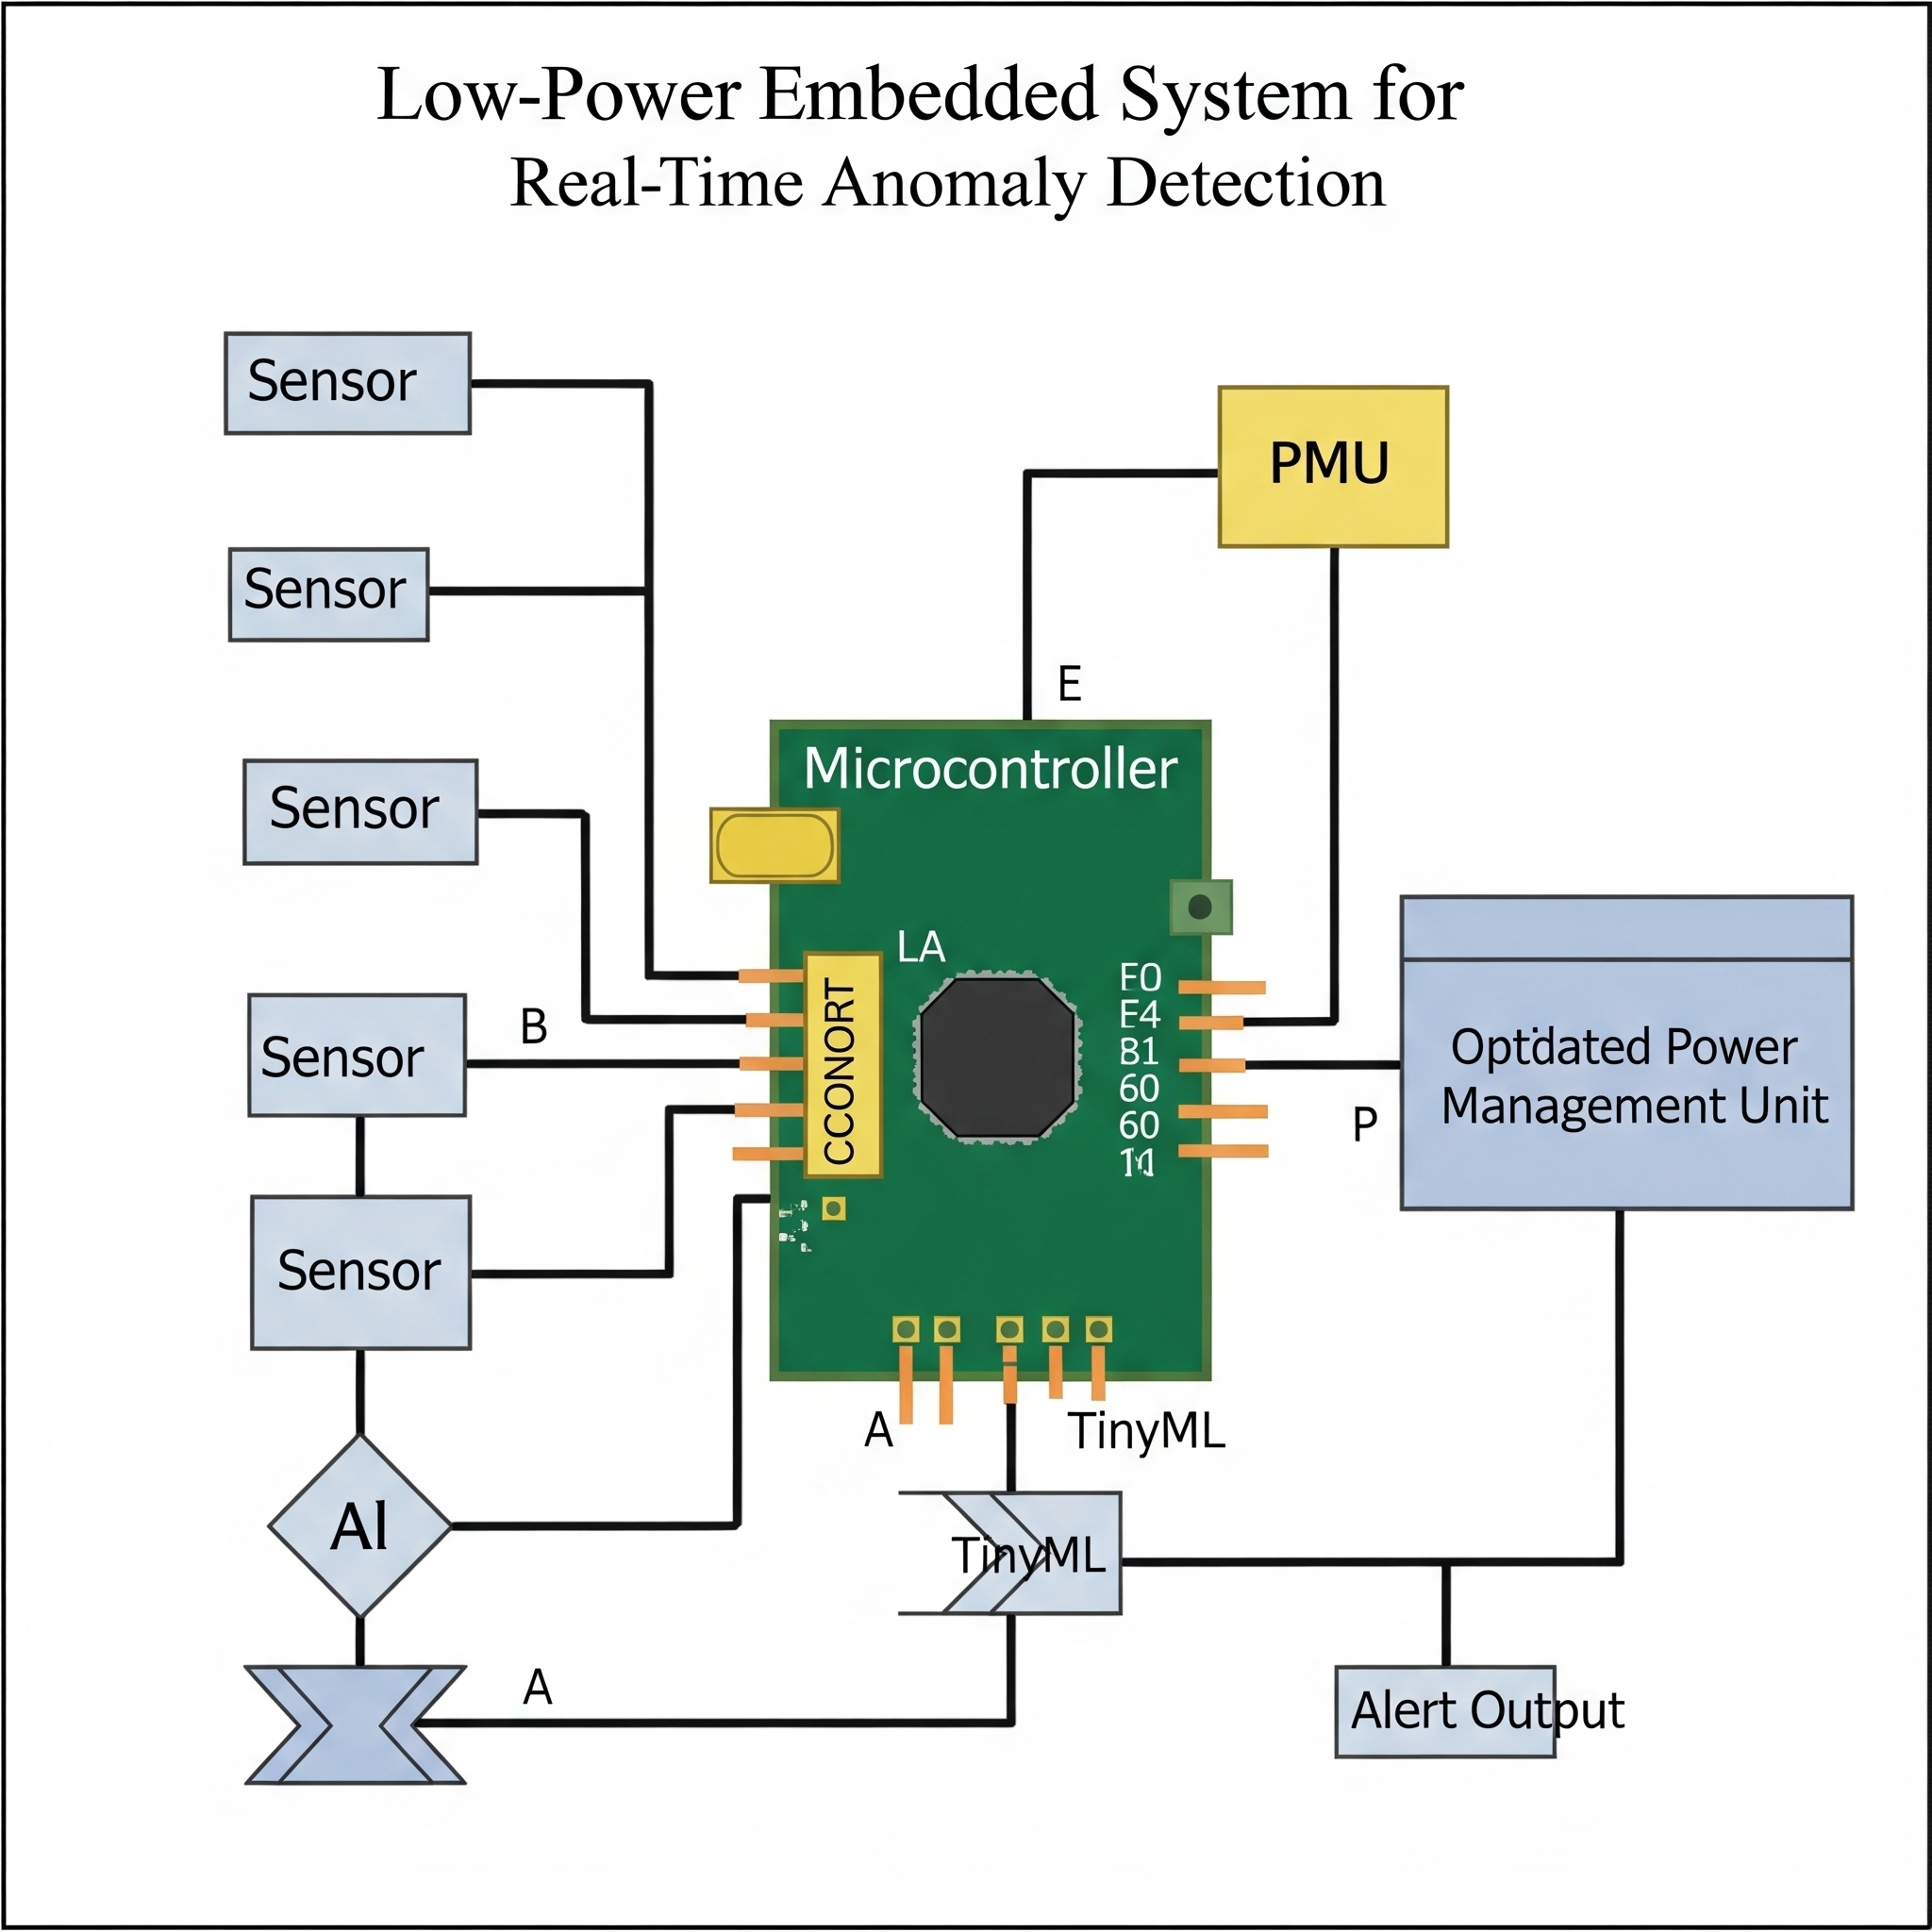
\includegraphics[width=0.65\textwidth]{fig/diagrama_sistema_ejemplo.png}
    \caption{Diagrama de bloques del sistema empotrado para detección de anomalías.}
    \label{fig:diagrama_ejemplo}
\end{figure}

\section{Inclusión de Tablas}
\label{sec:tablas}

Las tablas son una herramienta esencial para presentar datos de forma estructurada, clara y comparativa. En \LaTeX{}, las tablas se construyen generalmente utilizando el entorno \texttt{table}, que actúa como un contenedor flotante, junto con el entorno \texttt{tabular}, que es el encargado de organizar el contenido en filas y columnas.

Para garantizar una apariencia profesional y mejorar la legibilidad, esta plantilla incluye el paquete \texttt{booktabs}. Se recomienda encarecidamente utilizar sus comandos (\verb|\toprule|, \verb|\midrule| y \verb|\bottomrule|) para las líneas horizontales, ya que crean un espaciado más adecuado que el tradicional \verb|\hline|. Como norma general, es preferible evitar las líneas verticales para un diseño más limpio.

El siguiente código muestra cómo definir una tabla, asignarle un título y prepararla para ser referenciada:

\begin{verbatim}
\begin{table}[H]
    \centering
    \caption{Ejemplo de tabla formateada con el paquete booktabs.}
    \label{tab:ejemplo_consumo}
    \begin{tabular}{lcc}
        \toprule
        \textbf{Componente} & \textbf{Consumo (W)} & \textbf{Horas de uso} \\
        \midrule
        Lavadora & 2200 & 1.5 \\
        Lavavajillas & 1800 & 1.0 \\
        Cargador VE & 7400 & 3.0 \\
        \bottomrule
    \end{tabular}
\end{table}
\end{verbatim}

Los componentes clave son:
\begin{itemize}
    \item \verb|\begin{table}[H]|: Inicia el entorno flotante. Al igual que con las figuras, el especificador \texttt{[H]} del paquete \texttt{float} fuerza su aparición en ese punto exacto del texto, aunque se desaconseja su uso para permitir que \LaTeX{} optimice la maquetación.
    \item \verb|\centering|: Centra la tabla horizontalmente.
    \item \verb|\caption{...}|: Añade un título descriptivo y numerado que aparecerá encima de la tabla.
    \item \verb|\label{tab:ejemplo_consumo}|: Asigna un identificador único para poder referenciarla. Se recomienda usar el prefijo \texttt{tab:}.
    \item \verb|\begin{tabular}{lcc}|: Define la estructura de la tabla, en este caso con tres columnas: la primera alineada a la izquierda (\texttt{l}) y las otras dos centradas (\texttt{c}).
    \item \verb|\toprule|, \verb|\midrule|, \verb|\bottomrule|: Comandos de \texttt{booktabs} para las líneas superior, media e inferior, respectivamente.
\end{itemize}

Para hacer referencia a la tabla en el texto, se utiliza el comando \verb|\autoref{}|, que genera automáticamente la palabra "Tabla" seguida de su número y crea un hipervínculo.

\begin{verbatim}
En la \autoref{tab:ejemplo_consumo} se detallan los consumos de la \gls{cpu} 
del microcontrolador, según el modo de funcionamiento
\end{verbatim}

Vemos el ejemplo en uso a continuación: En la \autoref{tab:ejemplo_consumo} se detallan los consumos de la \gls{cpu} del microcontrolador, según el modo de funcionamiento.

\begin{table}
    \centering
    \caption{Ejemplo de tabla formateada con el paquete booktabs.}
    \label{tab:ejemplo_consumo}
    \begin{tabular}{lcc}
        \toprule
        \textbf{Modo} & \textbf{Consumo (mA)} & \textbf{Potencia (mW)} \\
        \midrule
        Activo & 50 & 165 \\
        Con WiFi & 250 & 825 \\
        Light Sleep & 1,2 & 3,96 \\
        \bottomrule
    \end{tabular}
\end{table}

\subsection{Tablas que ocupan varias páginas}
Si una tabla es demasiado extensa para caber en una sola página, el entorno \texttt{table} no es adecuado. Para estos casos, la plantilla carga el paquete \texttt{longtable}, que permite que las tablas se dividan y continúen en las páginas siguientes de forma automática, repitiendo la cabecera si así se especifica.

\section{Inclusión de Listados de Código}
\label{sec:listados_codigo}

Para presentar algoritmos o fragmentos de código fuente, la plantilla integra el paquete \texttt{listings}, que proporciona un entorno específico para formatear el código de manera clara y legible. Se ha preconfigurado un estilo visual consistente para asegurar que todos los listados de código mantengan una apariencia profesional y homogénea a lo largo del documento.

Para insertar un bloque de código, se utiliza el entorno \texttt{lstlisting}. Este entorno numera automáticamente los listados y les aplica el formato definido en la plantilla (resaltado de sintaxis, color de fondo, etc.).

El siguiente ejemplo muestra cómo incluir un listado de código, con su leyenda y etiqueta para poder ser referenciado posteriormente:

\begin{verbatim}
\begin{lstlisting}[language=Python, caption={Ejemplo de un listado de código en Python.}, label={lst:ejemplo_python}]
# Este es un comentario
def factorial(n):
    """
    Calcula el factorial de un número entero no negativo.
    """
    if n == 0:
        return 1
    else:
        return n * factorial(n - 1)

# Llamada a la función
resultado = factorial(5)
print(f"El factorial de 5 es {resultado}")
\end{lstlisting}
\end{verbatim}

Los componentes clave son:
\begin{itemize}
    \item \verb|\begin{lstlisting}[...]|: Inicia el entorno para el listado de código. Dentro de los corchetes se pueden especificar opciones importantes:
    \begin{itemize}
        \item \verb|language=...|: Define el lenguaje de programación (p. ej., \texttt{Python}, \texttt{C++}, \texttt{Java}, \texttt{SQL}, \texttt{XML}). Esto es crucial para que el paquete resalte la sintaxis correctamente.
        \item \verb|caption={...}|: Añade una leyenda descriptiva y numerada debajo del listado de código.
        \item \verb|label={...}|: Asigna un identificador único. Se recomienda usar el prefijo \texttt{lst:} para evitar confusiones con otras etiquetas.
    \end{itemize}
    \item \verb|\end{lstlisting}|: Finaliza el entorno del listado de código.
\end{itemize}

Una vez que el listado ha sido etiquetado con \verb|\label|, puedes hacer referencia a él en el texto utilizando el comando \verb|\autoref{}|. De forma similar a las figuras y tablas, este comando generará automáticamente el tipo de elemento y su número (p. ej., "Listado 1.1"), creando además un hipervínculo.

Por ejemplo, para citar el listado anterior, escribirías:
\begin{verbatim}
En el \autoref{lst:ejemplo_python} se muestra una función para calcular el 
factorial.
\end{verbatim}

Que viene a quedar como sigue: En el \autoref{lst:ejemplo_python} se muestra una función para calcular el factorial.

\begin{lstlisting}[language=Python, caption={Ejemplo de un listado de código en Python.}, label={lst:ejemplo_python}]
# Este es un comentario
def factorial(n):
    """
    Calcula el factorial de un número entero no negativo.
    """
    if n == 0:
        return 1
    else:
        return n * factorial(n - 1)

# Llamada a la función
resultado = factorial(5)
print(f"El factorial de 5 es {resultado}")
\end{lstlisting}

\section{Uso de Ecuaciones}
Las ecuaciones son cruciales para expresar formalmente conceptos matemáticos, modelos y algoritmos. LaTeX ofrece varias formas de incluir ecuaciones, ya sea en línea con el texto o como elementos separados y numerados.

\subsection{Ecuaciones en línea}
Para incluir ecuaciones pequeñas directamente dentro de una frase, se utiliza el modo matemático en línea, delimitado por signos de dólar (\verb|$|). Por ejemplo, para expresar la famosa ecuación de Einstein, escribiríamos \verb|$E=mc^2$|, que se verá como $E=mc^2$. Este método es útil para fórmulas cortas que no necesitan una numeración o un espacio dedicado.

\subsection{Ecuaciones numeradas y centradas}
Cuando una ecuación es más compleja, necesita destacarse del texto, o se desea referenciarla posteriormente, se utiliza el entorno \texttt{equation}. Este entorno centra la ecuación automáticamente y le asigna un número secuencial.

El siguiente ejemplo muestra cómo definir una ecuación:
\begin{verbatim}
\begin{equation}\label{eq:parabola}
    y = ax^2 + bx + c
\end{equation}
\end{verbatim}

Los componentes clave son:
\begin{itemize}
    \item \verb|\begin{equation}|: Inicia el entorno de ecuación.
    \item \verb|\label{eq:parabola}|: Asigna un identificador único a la ecuación. Se recomienda usar el prefijo \texttt{eq:} para evitar confusiones con otras etiquetas.
\end{itemize}

Para hacer referencia a esta ecuación en el texto, se utiliza el comando \verb|\eqref{}|. Este comando genera automáticamente el número de la ecuación entre paréntesis (p.ej., ``(1.1)'') y crea un hipervínculo. Por ejemplo:

En \eqref{eq:parabola} se muestra la ecuación general de una parábola.

\begin{equation}\label{eq:parabola}
    y = ax^2 + bx + c
\end{equation}

\subsection{Sistemas de ecuaciones}
Para sistemas de ecuaciones, el entorno \texttt{eqnarray} es una opción que permite alinear múltiples ecuaciones. Sin embargo, se recomienda el uso del paquete \texttt{amsmath} y sus entornos como \texttt{align} o \texttt{gather} para una mayor flexibilidad y un mejor espaciado.

Aquí se muestra un ejemplo básico con \texttt{eqnarray} (aunque se sugiere \texttt{amsmath} para casos más avanzados):

\begin{verbatim}
\begin{eqnarray}\label{eq:sistema_ecuaciones}
    2x + 3y &=& 7 \\
    x - y &=& 1
\end{eqnarray}
\end{verbatim}

Este código produce el siguiente sistema de ecuaciones:

\begin{eqnarray}\label{eq:sistema_ecuaciones}
    2x + 3y &=& 7 \\
    x - y &=& 1
\end{eqnarray}

Se puede hacer referencia a este sistema de la misma manera que una ecuación individual, por ejemplo, utilizando la ecuación \eqref{eq:sistema_ecuaciones}.

\chapter{Resto de capítulos}
Aquí irían el resto de capítulos. Generalmente \emph{Estado del arte}, \emph{Metodología}, y \emph{Experimentos y resultados}, por poner un ejemplo.

\chapter{Conclusiones y trabajo futuro}
Aquí van las conclusiones y trabajo futuro.

\chapter{Introduction}
Traduce aquí tu capítulo de introducción.

\chapter{Conclusion and future work}
Traduce aquí tu capítulo de conclusiones y trabajo futuro.

%Bibliografia
\bibliographystyle{IEEEtran}
\bibliography{biblio}\addcontentsline{toc}{chapter}{Bibliografía}

\printglossary[type=\acronymtype, title={Acrónimos}]

\end{document}
